%============ Chapter3.tex — Methodology ===================
\chapter{Methodology}

\section{Overview}

This chapter specifies the complete system, from the raw audio file to
the cautious screening indication, in the order in which data flows
through it. Two principles govern every design decision and are worth
stating before the details. The first is the \emph{same-pipeline rule}:
the identical preprocessing, segmentation, and feature-extraction code
is used for training, for evaluation, and for predicting on a new
file, and this identity is enforced mechanically rather than by
convention. The second is \emph{subject independence}: no data derived
from a given person is ever allowed to influence a model that is
evaluated on that person, and this too is enforced by the code itself.

Sections~3.2--3.6 describe the data path: system architecture, the
dataset and its inspection, preprocessing, segmentation, and feature
extraction. Sections~3.7--3.9 describe the modelling side: the
classification pipeline, the validation protocol, and the pre-declared
model-selection rules. Section~3.10 specifies the external validation
design, Section~3.11 the prototype, and Section~3.12 the software
environment and reproducibility measures.

\section{System Architecture}

Figure~\ref{fig:pipeline} shows the complete processing chain. A
recording is first conditioned by a five-step preprocessing stage, then
divided into 10-second chunks. From every chunk, 74 acoustic features
are extracted; the recording is represented by the per-feature mean
over its chunks. This vector enters a classification pipeline
consisting of a median imputer, a standard scaler, and the classifier,
which outputs a score between 0 and 1 for the PD class. Finally, an
interpretation stage maps the score to one of three outcomes ---
closer to the Healthy Control (HC) class, closer to the PD class, or
inconclusive --- and attaches any recording-condition warnings and the
mandatory non-diagnostic wording.

\begin{figure}[htb]
\centering
\begin{tikzpicture}[
  font=\small,
  box/.style={draw, rounded corners=2pt, minimum width=2.55cm,
              minimum height=1.05cm, align=center, thick},
  note/.style={font=\footnotesize\itshape, align=center},
  arr/.style={-{Stealth[length=2.6mm]}, thick}
]
\node[box] (wav) {Raw WAV\\recording};
\node[box, right=7mm of wav] (pre) {Preprocessing\\{\footnotesize 5 steps}};
\node[box, right=7mm of pre] (seg) {Segmentation\\{\footnotesize 10-s chunks}};
\node[box, right=7mm of seg] (feat) {Feature\\extraction\\{\footnotesize 74 / chunk}};
\node[box, below=9mm of feat] (agg) {Chunk-mean\\aggregation};
\node[box, left=7mm of agg] (clf) {Imputer $\to$ scaler\\$\to$ classifier};
\node[box, left=7mm of clf] (interp) {Score\\interpretation};
\node[box, left=7mm of interp] (out) {Non-diagnostic\\indication};
\draw[arr] (wav) -- (pre);
\draw[arr] (pre) -- (seg);
\draw[arr] (seg) -- (feat);
\draw[arr] (feat) -- (agg);
\draw[arr] (agg) -- (clf);
\draw[arr] (clf) -- (interp);
\draw[arr] (interp) -- (out);
\node[note, below=2mm of interp] {inconclusive band,\\condition warnings};
\node[note, below=2mm of clf] {fitted on training\\folds only};
\end{tikzpicture}
\caption{The complete processing chain. The same implementation of
every stage is shared by training, evaluation, and prediction.}
\label{fig:pipeline}
\end{figure}

All numerical settings of every stage --- sample rate, trimming
threshold, pitch search range, segmentation lengths, spectral analysis
parameters --- are defined once in a single configuration module. When
a model is trained, the full configuration, including the complete
ordered list of feature names, is saved beside the model as a
machine-readable contract. Before \emph{every} prediction, the software
compares this saved contract with the configuration of the running
code; any difference, or a missing contract file, aborts the prediction
with an instruction to retrain. The same-pipeline rule is therefore a
verified property of the system, not a development convention.

\section{Dataset and Inspection Protocol}

\subsection{The MDVR-KCL Corpus}

The training corpus is the MDVR-KCL database \cite{jaeger2019},
comprising smartphone voice recordings of English-speaking participants
performing two tasks: reading a fixed text (ReadText) and holding a
spontaneous conversation (SpontaneousDialogue). Table~\ref{tab:dataset}
summarizes its composition as verified by the inspection stage. All
73 recordings are mono WAV files sampled at 44100~Hz, with durations
between 73.0 and 220.6 seconds (median 141.3~s). Each participant
contributed at most one recording per task; 36 of the 37 subjects have
exactly two recordings, and one PD subject has one.

\begin{table}[htb]
\centering
\caption{Composition of the MDVR-KCL corpus as used in this project.}
\label{tab:dataset}
\begin{tabular}{lccc}
\toprule
Group & Subjects & ReadText & SpontaneousDialogue \\
\midrule
Healthy Control (HC) & 21 & 21 & 21 \\
Parkinson's Disease (PD) & 16 & 16 & 15 \\
\midrule
Total & 37 & 37 & 36 \\
\bottomrule
\end{tabular}
\end{table}

\subsection{Labels and Subject Identities}

The class label of each file is determined from two independent
sources: the folder in which the file resides (HC or PD) and a tag
embedded in its filename. The two sources are cross-checked, and a file
whose sources disagree would be excluded and reported as a label
conflict rather than assigned silently; no such conflict occurred. The
subject identity is parsed from the leading identifier token of the
filename. This identity is the basis of subject-independent validation,
so files without a recognizable subject identifier would likewise be
excluded and reported; none occurred.

\subsection{Integrity Checks}

Before any modelling, an automated inspection verified: readability of
every file; absence of empty, silent, or very short recordings;
absence of duplicate audio content (by MD5 hash comparison, which
protects against the same recording entering both training and test
data under different names); label consistency; and absence of
subjects appearing in more than one class. All 73 files passed every
check. The inspection also recorded the dataset's known risks --- small
sample size, homogeneous recording conditions, class imbalance (42 HC
versus 31 PD recordings), and the absence of per-subject demographic
metadata --- which shape the validation and analysis decisions
described below.

\section{Audio Preprocessing}

Each recording passes through five conditioning steps, in fixed order:

\begin{enumerate}
  \item \textbf{Mono conversion.} Multi-channel input is averaged to a
        single channel.
  \item \textbf{Resampling to 44100~Hz.} All analysis assumes one fixed
        sample rate; 44100~Hz is the native rate of the corpus, so no
        resampling artefacts are introduced for the training data.
  \item \textbf{DC-offset removal.} The signal mean is subtracted; a
        constant offset would bias amplitude-based measures such as
        shimmer.
  \item \textbf{Edge silence trimming.} Leading and trailing segments
        more than 30~dB below the signal peak are removed. Internal
        pauses are deliberately retained, both because the pause
        features measure them and because cutting inside the recording
        would create artificial amplitude discontinuities.
  \item \textbf{Peak normalization.} The signal is scaled so that its
        maximum absolute amplitude is 0.95, making recordings
        comparable across input gains. Because jitter, shimmer, and the
        other perturbation measures are relative quantities
        (Eqs.~2.1--2.2), a uniform gain change does not distort them.
\end{enumerate}

No denoising, filtering, or spectral enhancement of any kind is
applied. This is a deliberate scientific decision: noise-reduction
algorithms operate precisely by detecting and suppressing signal
irregularities, and cycle-to-cycle irregularity is exactly the clinical
information that jitter, shimmer, HNR, and CPPS are designed to
measure. Aggressive cleaning would make a disordered voice appear
artificially healthy.

\section{Segmentation and Aggregation}

After preprocessing, each recording is divided into consecutive
non-overlapping chunks of 10~seconds; a trailing chunk shorter than
5~seconds is discarded, and a recording shorter than the chunk length
is processed as a single chunk. Applied to the corpus, this produced
1001 chunks (between 7 and 22 per recording).

Features are extracted per chunk, and the recording-level feature
vector is the per-feature arithmetic mean over its $K$ chunks:
\begin{equation}
\bar{x}_j \;=\; \frac{1}{K}\sum_{k=1}^{K} x_{j,k},
\qquad j = 1,\dots,74,
\label{eq:chunkmean}
\end{equation}
where $x_{j,k}$ is feature $j$ measured on chunk $k$. Averaging many
short-window measurements is statistically more stable than one
measurement over a whole recording, and the experiments of Chapter~4
show that this representation improves classification. The chunks
inherit the recording's subject identity, so the grouping required for
honest validation is preserved --- and Section~3.8 shows what happens
when it is not.

\section{Feature Extraction}

Table~\ref{tab:features} lists the eight feature families; their
definitions and physiological meaning were given in Section~2.4. The
complete inventory of all 74 names appears in Appendix~A.

\begin{table}[htb]
\centering
\caption{The 74 acoustic features extracted from every chunk.}
\label{tab:features}
\begin{tabular}{lcl}
\toprule
Family & Count & Tool \\
\midrule
F0 statistics & 7 & Praat via Parselmouth \\
Jitter variants & 4 & Praat via Parselmouth \\
Shimmer variants & 5 & Praat via Parselmouth \\
Harmonics-to-noise ratio & 1 & Praat via Parselmouth \\
Smoothed cepstral peak prominence & 1 & Praat via Parselmouth \\
Pause and timing statistics & 4 & energy-based segmentation \\
MFCC summary statistics & 26 & librosa \\
Delta-MFCC summary statistics & 26 & librosa \\
\midrule
Total & 74 & \\
\bottomrule
\end{tabular}
\end{table}

The principal analysis settings are as follows. Pitch tracking and the
perturbation measures use the autocorrelation method \cite{boersma1993}
with a search range of 75--500~Hz. CPPS uses Praat's power-cepstrogram
analysis with a 60~Hz pitch floor, a 2~ms time step, and a peak search
range of 60--330~Hz. Pause statistics use an energy threshold of 25~dB
below peak with a minimum pause duration of 0.2~s. MFCC analysis uses
13 coefficients over 2048-sample windows with a 512-sample hop
(approximately 46~ms and 12~ms at 44100~Hz), summarized by mean and
standard deviation per coefficient, and likewise for their time
derivatives \cite{davis1980,mcfee2015}.

On chunks containing too little stable voicing, Praat cannot compute
some perturbation measures; these values are recorded as missing rather
than fabricated. In the corpus this affected at most 16 of the 1001
chunks for any single feature. Missing values are filled by the median
imputer of the classification pipeline, which --- critically --- is
fitted inside each training fold only (Section~3.7).

The extraction stage always computes all 74 features through a single
code path; the original 43-feature set of the baseline phase
(Chapter~4) is a named subset of the same table, so base and extended
experiments differ only in column selection, never in extraction code.

\section{Classification Pipeline}

Every classifier is embedded in a three-stage pipeline executed as one
object:
\begin{center}
median imputer \; $\to$ \; standard scaler \; $\to$ \; classifier
\end{center}
The imputer replaces missing values with the median of the
corresponding feature. The scaler standardizes each feature to zero
mean and unit variance,
\begin{equation}
z_j = \frac{x_j - \mu_j}{\sigma_j},
\label{eq:zscore}
\end{equation}
which is necessary because the features span incommensurate scales
(mean F0 is of order $10^2$~Hz while local jitter is of order
$10^{-2}$). Both stages estimate their statistics
($\mu_j$, $\sigma_j$, medians) \emph{from the training portion of each
validation fold only}; embedding them in the pipeline object guarantees
this and thereby closes the preprocessing leakage channel described in
Section~2.6.

Five models are trained and compared, all implemented in scikit-learn
\cite{pedregosa2011}: a majority-class baseline; logistic regression
(maximum 5000 iterations); an SVM with RBF kernel \cite{cortes1995};
a Random Forest of 300 trees with unrestricted depth
\cite{breiman2001}; and an MLP with hidden layers of 32 and 16 units.
All models except the baseline use balanced class weighting, which
scales each training example inversely to its class frequency so that
the minority PD class is not systematically under-predicted. A fixed
random seed makes every training run reproducible.

\section{Subject-Independent Validation Protocol}

\subsection{Grouped Cross-Validation}

Evaluation uses stratified grouped 5-fold cross-validation, with the
subject identity as the grouping variable, repeated with three random
seeds (42, 7, and 2025). The grouped splitter assigns all recordings
(and therefore all chunks) of one subject to the same side of every
split, while stratification keeps the HC/PD proportion approximately
constant across folds. Figure~\ref{fig:groupedcv} illustrates the
principle. Within each of the $3\times5$ evaluations, the model is
fitted on the training subjects and produces predictions for the held-%
out subjects; collecting these across folds yields exactly one
\emph{out-of-fold} prediction per recording per seed, made in every
case by a model that never saw that person.

\begin{figure}[htb]
\centering
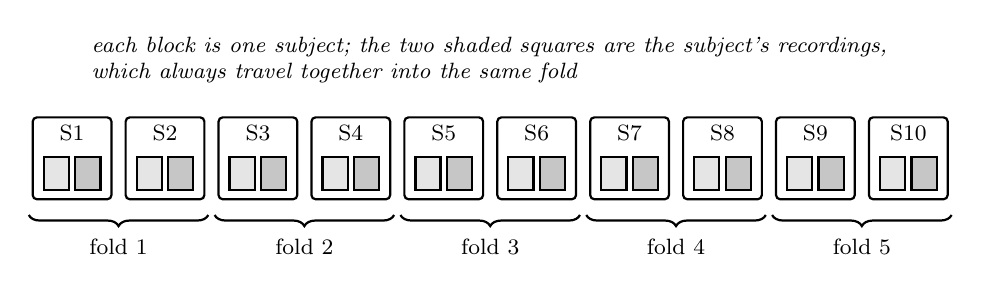
\begin{tikzpicture}[font=\footnotesize, thick]
% subjects as pairs of recordings
\foreach \i/\c in {0/f1,1/f1,2/f2,3/f2,4/f3,5/f3,6/f4,7/f4,8/f5,9/f5}{
  \begin{scope}[shift={(\i*1.18,0)}]
    \draw[rounded corners=1.5pt] (-0.5,-0.42) rectangle (0.5,0.62);
    \node at (0,0.42) {S\the\numexpr\i+1\relax};
    \draw[fill=gray!20] (-0.36,-0.3) rectangle (-0.04,0.12);
    \draw[fill=gray!45] (0.04,-0.3) rectangle (0.36,0.12);
  \end{scope}
}
\draw[decorate, decoration={brace, mirror, amplitude=4pt}]
  (-0.55,-0.62) -- (1.73,-0.62) node[midway, below=5pt] {fold 1};
\draw[decorate, decoration={brace, mirror, amplitude=4pt}]
  (1.81,-0.62) -- (4.09,-0.62) node[midway, below=5pt] {fold 2};
\draw[decorate, decoration={brace, mirror, amplitude=4pt}]
  (4.17,-0.62) -- (6.45,-0.62) node[midway, below=5pt] {fold 3};
\draw[decorate, decoration={brace, mirror, amplitude=4pt}]
  (6.53,-0.62) -- (8.81,-0.62) node[midway, below=5pt] {fold 4};
\draw[decorate, decoration={brace, mirror, amplitude=4pt}]
  (8.89,-0.62) -- (11.17,-0.62) node[midway, below=5pt] {fold 5};
\node[align=left, font=\footnotesize\itshape] at (5.3,1.35)
  {each block is one subject; the two shaded squares are the subject's
   recordings,\\which always travel together into the same fold};
\end{tikzpicture}
\caption{Subject-grouped cross-validation (illustrated with 10
subjects). A subject's recordings are never divided between training
and test folds.}
\label{fig:groupedcv}
\end{figure}

The splitter's guarantee is not taken on trust. Inside every fold, the
implementation recomputes the intersection of training and test
subjects and halts the program if it is non-empty:

\begin{verbatim}
overlap = set(groups[train_idx]) & set(groups[test_idx])
if overlap:
    raise RuntimeError(f"LEAKAGE: subjects {overlap} "
                        "appear in train AND test")
\end{verbatim}

\noindent
This assertion never triggered in any experiment of this project.

Results are reported at two levels. The \emph{recording level} scores
each audio file independently. The \emph{subject level} averages the
out-of-fold PD scores of a subject's recordings and applies the 0.5
threshold to the mean; it is the clinically more relevant level, since
the practical question concerns persons, not files. All headline
metrics are stated as mean $\pm$ standard deviation over the three
seeds.

\subsection{Metrics}

With TP, TN, FP, and FN denoting true positives (PD correctly
identified), true negatives, false positives, and false negatives, the
reported metrics are:
\begin{align}
\text{sensitivity} &= \frac{\mathrm{TP}}{\mathrm{TP}+\mathrm{FN}},
\qquad
\text{specificity} = \frac{\mathrm{TN}}{\mathrm{TN}+\mathrm{FP}},
\label{eq:sensspec}\\[4pt]
\text{balanced accuracy} &=
\tfrac{1}{2}\left(\text{sensitivity}+\text{specificity}\right),
\label{eq:balacc}\\[4pt]
\text{precision} &= \frac{\mathrm{TP}}{\mathrm{TP}+\mathrm{FP}},
\qquad
F_1 = \frac{2\,(\text{precision}\times\text{sensitivity})}
           {\text{precision}+\text{sensitivity}}.
\label{eq:f1}
\end{align}
Balanced accuracy is the primary metric because the classes are
imbalanced: a baseline that always answers HC attains
$42/73 \approx 0.575$ plain accuracy while detecting no patient at
all, but only 0.5 balanced accuracy, which correctly exposes it.
Confusion matrices are reported for all models. In addition, the Area
Under the Receiver Operating Characteristic Curve (AUC) summarizes the
model's scores independently of the 0.5 threshold; it equals the
probability that a randomly chosen PD case receives a higher score
than a randomly chosen HC case, with 0.5 corresponding to chance and
1.0 to perfect ranking.

Finally, a pre-declared warning rule guards against too-good-to-be-true
results: any subject-independent accuracy, balanced accuracy, or AUC
reaching 0.95 triggers an explicit investigation for leakage,
duplicates, or confounding before the result may be reported as a
success.

\section{Pre-Declared Model-Selection Protocol}

The accuracy-improvement study of Chapter~4 compares data
representations and models. Because repeatedly evaluating variants on
the same validation data can itself overfit --- the selection, rather
than the model, adapts to the data --- the following rules were fixed
\emph{before} any experiment was run:

\begin{enumerate}
  \item All variants are evaluated with the identical protocol of
        Section~3.8 (same folds, same three seeds).
  \item The primary metric is subject-level balanced accuracy, averaged
        over seeds.
  \item A more complex variant is adopted only if it exceeds the
        simpler alternative by more than 0.02 on the primary metric;
        otherwise the simpler variant is retained. The margin reflects
        the seed-to-seed variability observed at this sample size
        (about $\pm0.03$), below which differences are
        indistinguishable from noise.
  \item Any result at or above 0.95 halts the study for a leakage
        investigation (Section~3.8.2).
  \item Every evaluated configuration is reported, including rejected
        ones.
\end{enumerate}

Table~\ref{tab:variants} lists the seven data-representation variants
evaluated under these rules. Hyperparameter tuning (variant V4) is
performed by \emph{nested} grouped search: within each outer training
fold, an inner 3-fold grouped cross-validation selects, by balanced
accuracy, the SVM cost and kernel width
($C \in \{0.1, 1, 10, 100\}$,
$\gamma \in \{\text{scale}, 0.01, 0.001\}$), the RF depth and feature
fraction (depth $\in \{\text{unrestricted}, 5, 10\}$, features per
split $\in \{\sqrt{p}, 0.3p\}$), and the logistic-regression
regularization ($C \in \{0.01, 0.1, 1, 10\}$); the outer test subjects
play no role in the choice. The ensemble (V5) soft-votes the
per-fold-tuned SVM and RF.

\begin{table}[htb]
\centering
\caption{Data-representation variants of the model-selection study.}
\label{tab:variants}
\begin{tabular}{clc}
\toprule
Variant & Representation & Features \\
\midrule
V0 & whole-recording features (baseline phase) & 43 \\
V1 & chunk features averaged per recording (Eq.~\ref{eq:chunkmean}) & 74 \\
V2 & chunk-level classification, scores averaged & 43 \\
V3 & chunk-level classification, scores averaged & 74 \\
V4 & best of V0--V3 with nested hyperparameter tuning & --- \\
V5 & tuned SVM + RF soft-voting ensemble & --- \\
V6 & chunks summarized by mean and standard deviation & 148 \\
\bottomrule
\end{tabular}
\end{table}

\section{External Validation Design}

The final model is additionally evaluated on the Italian Parkinson's
Voice and Speech database \cite{dimauro2017}, under a design agreed
before the evaluation was run:

\begin{enumerate}
  \item \textbf{Inspection first.} The external corpus undergoes the
        same automated inspection as the training corpus before any
        evaluation, covering structure, speaker identities, formats,
        sample rates, and durations. As Chapter~4 reports, this step
        uncovered a systematic association between sample rate and
        class that would otherwise have contaminated the result.
  \item \textbf{Inclusion rule.} Only recordings of at least
        30~seconds --- the continuous read-speech tasks --- are
        evaluated, because the short vowel and syllable tasks of that
        corpus do not match the continuous-speech conditions the
        pipeline is built for. The rule admits 216 recordings from all
        61 speakers of the mirrored corpus.
  \item \textbf{Bandwidth harmonization.} Every included file is first
        downsampled to 16~kHz --- removing all content above 8~kHz for
        every speaker equally --- and then resampled to the pipeline's
        standard 44100~Hz, after which the standard pipeline runs
        unchanged. This neutralizes the sample-rate confound
        identified during inspection.
  \item \textbf{Frozen model.} The classifier trained on MDVR-KCL is
        applied without any retraining, threshold adjustment, or
        adaptation. Speaker-level scores are formed exactly as in
        Section~3.8 (mean over the speaker's recordings, threshold
        0.5).
  \item \textbf{Age-fair comparison.} The headline result compares
        elderly healthy controls against the (elderly) PD group; the
        young control group is reported separately, since comparing
        young controls with elderly patients would confound age with
        disease.
  \item \textbf{Uncertainty reporting.} The fraction of results falling
        in the prototype's inconclusive band is reported alongside the
        metrics.
\end{enumerate}

\section{Prototype Design}

\subsection{Interfaces and Shared Prediction Path}

The prototype offers two interfaces: a browser application (built with
Streamlit \cite{streamlit}) supporting file upload and microphone
recording, and a command-line tool suited to scripted use. Both call
the same prediction function, which executes the pipeline of
Figure~\ref{fig:pipeline}; the interfaces therefore cannot diverge in
behaviour, and the automated tests of the prediction function cover
both.

Before every prediction, the saved pipeline contract
(Section~3.2) is verified. The input file is then validated with
plain-language rejection messages for each failure category: missing
file, empty file, undecodable audio, audio without samples, recordings
shorter than one second, and silent recordings.

\subsection{Score Interpretation and the Inconclusive Band}

The classifier's PD score is not presented as a bare class label.
Scores in the interval $[0.35, 0.65]$ are reported as inconclusive:
``the research model could not clearly assign this recording to either
class''. Scores outside the band are reported as ``the acoustic
pattern was classified by the research model as closer to the PD (or
HC) class''. Figure~\ref{fig:band} shows the decision rule. The band
exists because scores near the threshold carry weak evidence, and
because out-of-domain recordings --- different microphones, rooms, or
languages --- concentrate near the boundary, as the external
validation confirms; a hard label in that region would overstate what
the model knows. The band's placement matches the region where the
out-of-fold score distributions of the two classes overlap
(Chapter~4).

\begin{figure}[htb]
\centering
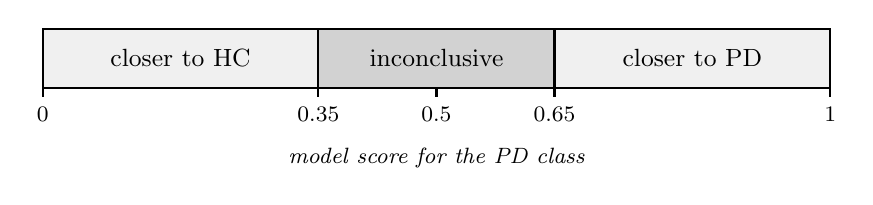
\begin{tikzpicture}[font=\small, thick]
\draw[fill=gray!12] (0,0) rectangle (3.5,0.75);
\draw[fill=gray!35] (3.5,0) rectangle (6.5,0.75);
\draw[fill=gray!12] (6.5,0) rectangle (10,0.75);
\draw (0,0) rectangle (10,0.75);
\node at (1.75,0.375) {closer to HC};
\node at (5,0.375) {inconclusive};
\node at (8.25,0.375) {closer to PD};
\foreach \x/\l in {0/0, 3.5/0.35, 5/0.5, 6.5/0.65, 10/1} {
  \draw (\x,0) -- (\x,-0.12) node[below, font=\footnotesize] {\l};
}
\node[below=18pt, font=\footnotesize\itshape] at (5,0)
  {model score for the PD class};
\end{tikzpicture}
\caption{Interpretation of the classifier score in the prototype.}
\label{fig:band}
\end{figure}

\subsection{Recording-Condition Warnings}

Non-blocking warnings accompany the result whenever the recording's
conditions depart from those of the training corpus: a native sample
rate different from 44100~Hz (the file is resampled, which can shift
spectral features); audible clipping (more than 0.1\% of samples at
full scale); an estimated Signal-to-Noise Ratio (SNR) below 15~dB,
computed from the ratio of the 90th to the 10th percentile of
Root Mean Square (RMS) frame energies over 50~ms frames; and analysed
durations under 10~seconds, far below the 70--220~s training
recordings. Microphone mode carries an additional standing notice that
live recordings differ from the training conditions and that the mode
mainly demonstrates the system's handling of unfamiliar input.

\subsection{Safety Wording and Data Handling}

Every result, in both interfaces, is framed by the mandatory
disclaimer: \emph{``This is a research screening-support prototype and
is not a medical diagnostic tool. Its result must not replace
evaluation by a qualified healthcare professional.''} The score is
explicitly labelled a property of the research model rather than a
person's medical risk, and the HC/PD labels are explained as
similarity to dataset groups. Uploaded or recorded audio is written
only to a temporary file that is deleted immediately after processing,
even on failure; no audio is retained. Unexpected internal errors are
never shown as technical traces: the user receives a short plain
message, while diagnostic detail is written to the terminal log (and,
in the command-line tool, exposed via a debug flag and distinct exit
codes).

\section{Development Environment and Tools}

The system is implemented in Python~3.14 inside a project-local
virtual environment. Praat \cite{boersma2001}, accessed through
Parselmouth \cite{jadoul2018}, computes the pitch, perturbation, HNR,
and CPPS measures; librosa \cite{mcfee2015} computes the MFCC family
and performs resampling and energy-based silence detection; NumPy
\cite{harris2020} and SciPy \cite{virtanen2020} provide numerical
routines; scikit-learn \cite{pedregosa2011} provides the models,
pipelines, and grouped splitters; Matplotlib \cite{hunter2007}
generates the result figures; and the pandas and SoundFile libraries
handle tabular data and audio input/output.

Reproducibility measures include: fixed random seeds throughout;
per-file caching of extracted features, so interrupted extraction runs
resume rather than restart; one script per pipeline stage, each
regenerating its report and artefacts from scratch; and version
control of all code, configuration, reports, and documentation in a
public repository (Appendix~C). The audio corpora themselves are not
redistributed --- they are excluded from the repository in accordance
with their licences, and download instructions are provided instead.
